\documentclass[t]{beamer}

\usetheme{Frankfurt}
%\usecolortheme{beaver}
\usefonttheme{professionalfonts}
% Insert the frame number at the bottom line
\expandafter\def\expandafter\insertshorttitle\expandafter{%
  \insertshorttitle\hfill\insertframenumber\,/\,\inserttotalframenumber}
% Remove the navigation symbols (one of the two options)
%\usenavigationsymbolstemplate{}
\setbeamertemplate{navigation symbols}{}

\usepackage{graphicx,color,dashbox,amsmath}
\usepackage{hyperref}% embedding hyperlinks [must be loaded after dropping]
\usepackage{amsmath}
\usepackage{amsthm,amssymb,amsfonts,latexsym,mathrsfs,wasysym}
\usepackage{pifont}
\usepackage{marvosym}
\usepackage{subfigure}
\usepackage{epstopdf}
\usepackage{soul,color}
\usepackage{threeparttable}% tables with footnotes
\usepackage{dcolumn}% decimal-aligned tabular math columns
\usepackage{float}
\usepackage{algorithm}
\usepackage{caption}
\usepackage[noend]{algpseudocode}
%\usepackage{subfig}

%\usepackage[style=ieee,backend=bibtex,citestyle=ieee]{biblatex}
%\usepackage[multiple]{footmisc}
%\addbibresource{bibliography.bib}
%\usepackage{colortbl}

\usepackage{tikz}
\usetikzlibrary{calc}
\usetikzlibrary{shapes.geometric}
\usetikzlibrary{arrows.meta}

%\usepackage{enumitem}
%\newlist{arrowlist}{itemize}{1}
%\setlist[arrowlist]{label=$\Rightarrow$}

\newcolumntype{d}{D{.}{.}{-1}}
\graphicspath{{Figures/}}

\logo{
\includegraphics[width=3em]{lapid-logo-45}}
\renewcommand{\baselinestretch}{1.2}

% commands and colors
\newcommand{\rR}{\mathbb{R}}
\newcommand{\rsqr}{\mathbb{R}^2}
\newcommand{\rthrd}{\mathbb{R}^3}
\newcommand{\eqsn}[1]{\begin{equation}#1\end{equation}}
\newcommand{\br}{$\\ $}

\newcommand{\bmat}[1]{\begin{bmatrix}#1\end{bmatrix}}
\newcommand{\mat}[1]{\begin{matrix}#1\end{matrix}}
\newcommand{\vmat}[1]{\begin{vmatrix}#1\end{vmatrix}}

\newcommand{\con}{c\left(t\right)}
\newcommand{\conp}[1]{c_{#1}\left(t\right)}
\newcommand{\concov}{\mathtt{C}\left(\con\right)}
\newcommand{\concovp}[1]{\mathtt{C}\left(\conp{#1}\right)}
\newcommand{\conset}{\mathtt{G}}

\newcommand{\sigp}{\sigma\left(p\right)}
\newcommand{\sigpp}[2]{\sigma_{#1 #2}\left(p \right)}
\newcommand{\pb}{\bar{p}}

\newcommand{\norm}[1]{\lVert #1 \rVert}

\makeatletter
\newcommand{\mathleft}{\@fleqntrue\@mathmargin0pt}
\newcommand{\mathcenter}{\@fleqnfalse}
\makeatother


% Gilad New Commands
\newcommand{\sgn}[1]{\operatorname{sgn}\left(#1\right)}
\newcommand{\sat}[1]{\operatorname{sat}\left(#1\right)}
%\newcommand{\rrule}[1]{\rule[#1]{0pt}{0pt}}

%beamer@blendedblue
\definecolor{mgreen}{RGB}{40,160,40}
\definecolor{natigreen}{RGB}{50,205,50}
\definecolor{natiblue}{RGB}{0,191,255}
\definecolor{mg}{rgb}{0,0.4,0}%
\definecolor{mypink2}{RGB}{219, 48, 122}

\newtheorem*{Proposition}{Proposition}
\newtheorem*{keylemma}{Key Lemma}
\newtheorem*{Remark}{Remark}
\newtheorem*{question}{Question}
\newtheorem*{Task}{Task}
\newtheorem*{cor}{Corollary}
\newtheorem*{thm}{Theorem}

%%%%%%%%%%%%%%%%%%%%%%%%%%

\title{A Projected Lloyd’s Algorithm for Coverage Control Problems}

\author[Palti]
{\Large Yoav Palti}

\institute[]
{Faculty of Aerospace Engineering, Technion - Israel Institute Of Technology}

\date[MSc Seminar]
{\footnotesize M.Sc. Seminar \\
Supervisor: Associate Professor Daniel Zelazo \\[1ex]
\em December 10, 2018}

\AtBeginSection[]
{
  \begin{frame}
    \frametitle{Table of Contents}
    \tableofcontents[currentsection]
  \end{frame}
}

\setbeamertemplate{blocks}[default]%[rounded][shadow=true]

%%%%%%%%%%%%%%%%%%%%%%%%%%
\begin{document}
\begingroup
% For the first slide only, remove all the text from the header/footer lines
\renewcommand*\insertshorttitle{}
\renewcommand*\insertshortauthor{}
\renewcommand*\insertshortinstitute{}
\renewcommand*\dohead{\rule{0em}{1.45em}}
\begin{frame}[label=sl1]
  \titlepage
\end{frame}
\endgroup

\begin{frame}
\frametitle{Table of Contents}
\tableofcontents
\end{frame}

%%%%%%%%%%%%%%%%%%%%%%%%%%%%%%%%%%%%%%%%%%
%%%%%%%%%%%%%% INTRODUCTION %%%%%%%%%%%%%%
%%%%%%%%%%%%%%%%%%%%%%%%%%%%%%%%%%%%%%%%%%

\section[Introduction]{Introduction}

%%% MOTIVATION %%%
\subsection[Motivation]{}
\begin{frame}[label=motivation1]{What Is Sensor Coverage?}
Given an area, we want to sense what's happening inside

\begin{figure}[b]
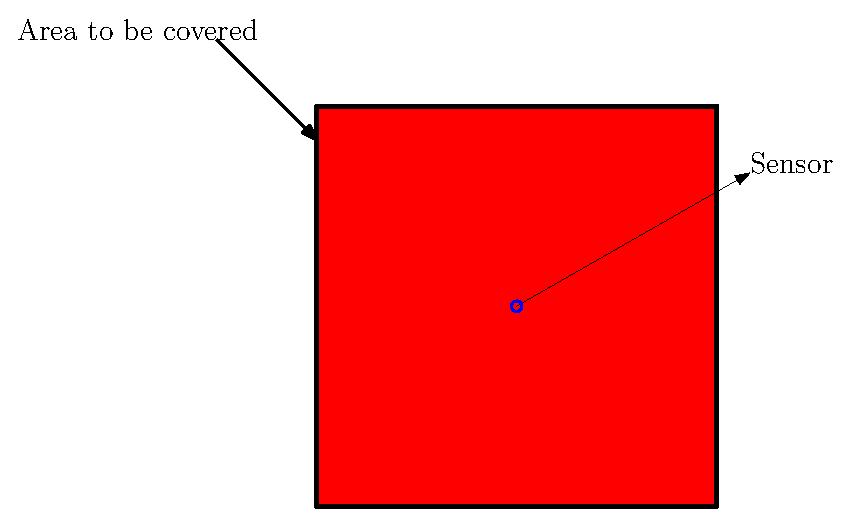
\includegraphics[scale=0.65]{motivation/coverage.eps}
\end{figure}
\end{frame}
%%
\begin{frame}[label=motivation2]{What Is Sensor Coverage?}
Why would we like to do that?
\begin{itemize}
\item Surveillance$^{1}$
\item Photographing$^{1}$
\item Exploring$^2$
\item iRobot!$^3$
\end{itemize}

\footnotetext[1]{\tiny Nigam, N., Bieniawski, S., Kroo, I., \& Vian, J. (2012). Control of multiple UAVs for persistent surveillance: Algorithm and flight test results. IEEE Transactions on Control Systems Technology, 20(5), 1236–1251.}
\footnotetext[2]{\tiny Loizou, S. G., \& Constantinou, C. C. (2016). Multi-Robot Coverage on Dendritic Topologies Under Communication Constraints, (Cdc).}
\footnotetext[3]{\tiny Montijano, E., Sagues, C., \& Llorente, S. (2016). Multi-Robot Persistent Coverage with Optimal Times, (Cdc), 3511–3517.}
\end{frame}
%%
\begin{frame}[label=motivation3]{What Is Sensor Coverage?}
Coverage "Capability" - how much a sensor can sense

\begin{figure}[b]
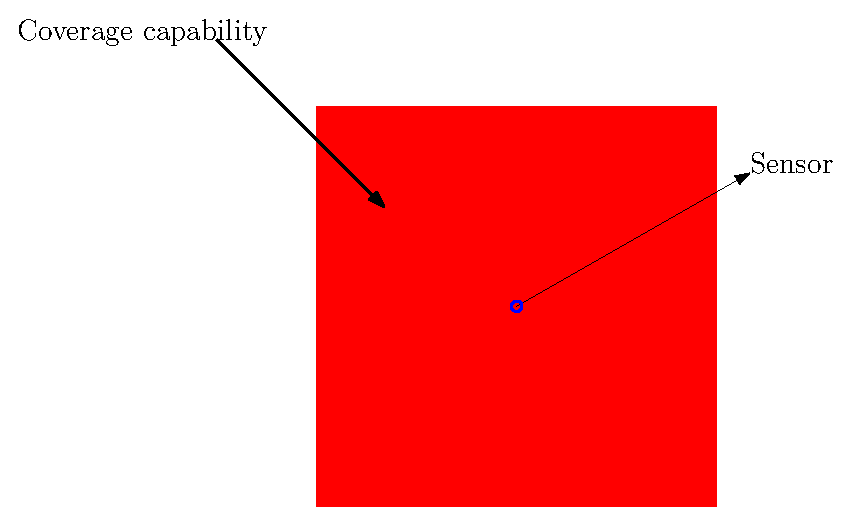
\includegraphics[scale=0.5]{motivation/coverage-radius.eps}
\end{figure}

In red - the sensor coverage \emph{Capability}. Most of the models refer the coverage capability as a circular area, thus it's also known as coverage \emph{radius}.
\end{frame}
%%
\begin{frame}[label=motivation4]{Partial Coverage}
Single sensor - double the area size

\begin{figure}[b]
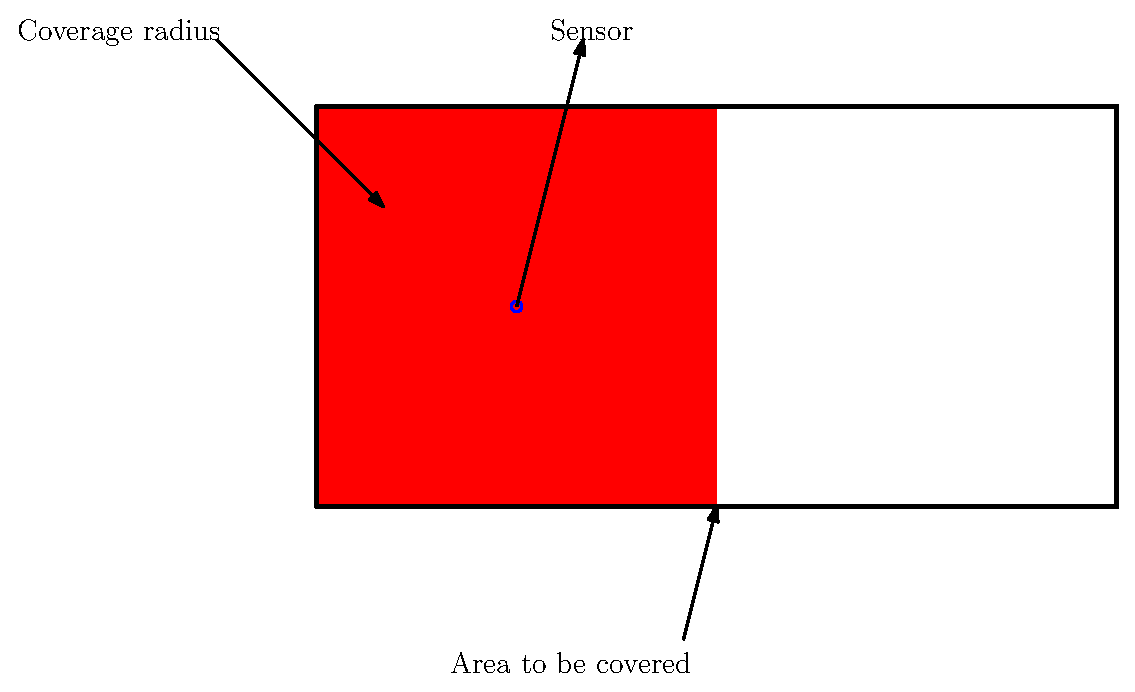
\includegraphics[scale=0.5]{motivation/partial-coverage.eps}
\end{figure}
In red - the sensor coverage. No \emph{full coverage}!
\end{frame}
%%
\begin{frame}[label=motivation5]{Full Coverage (again)}
Let's add another sensor!

\begin{figure}[b]
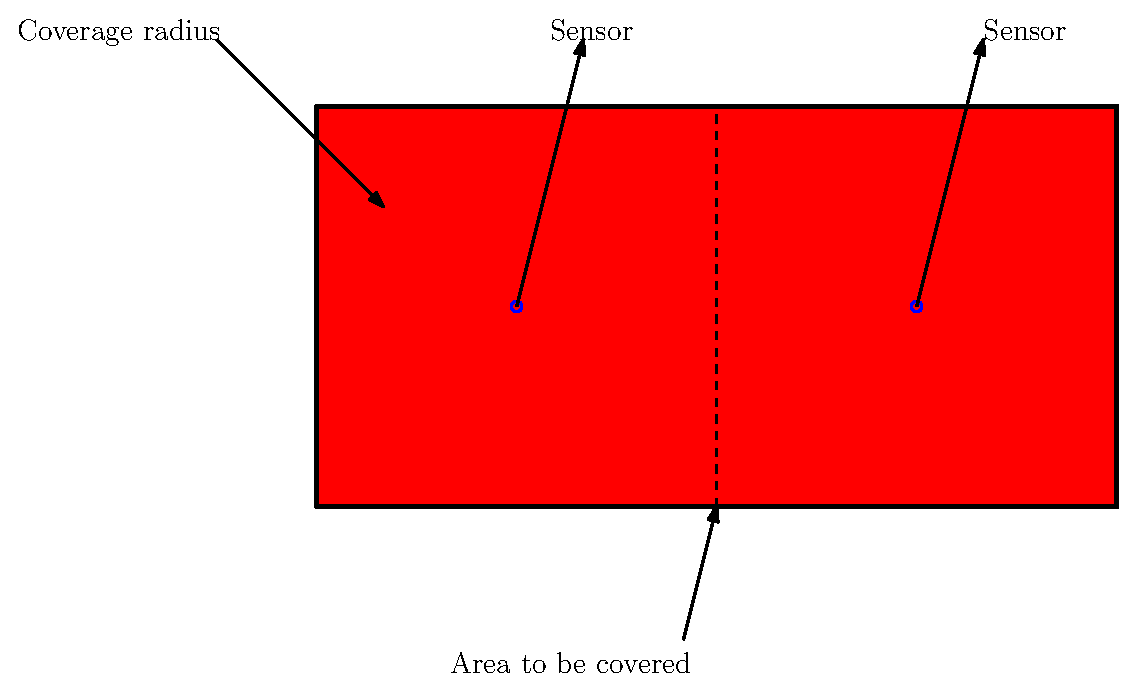
\includegraphics[scale=0.5]{motivation/partial-coverage-to-full.eps}
\end{figure}
New sensor added - now we have \emph{full coverage} once again!
\end{frame}
%%
\begin{frame}[label=motivation6]{Deployment}
Now we're dealing with multiple sensors. How should we configure them?

\begin{figure}[b]
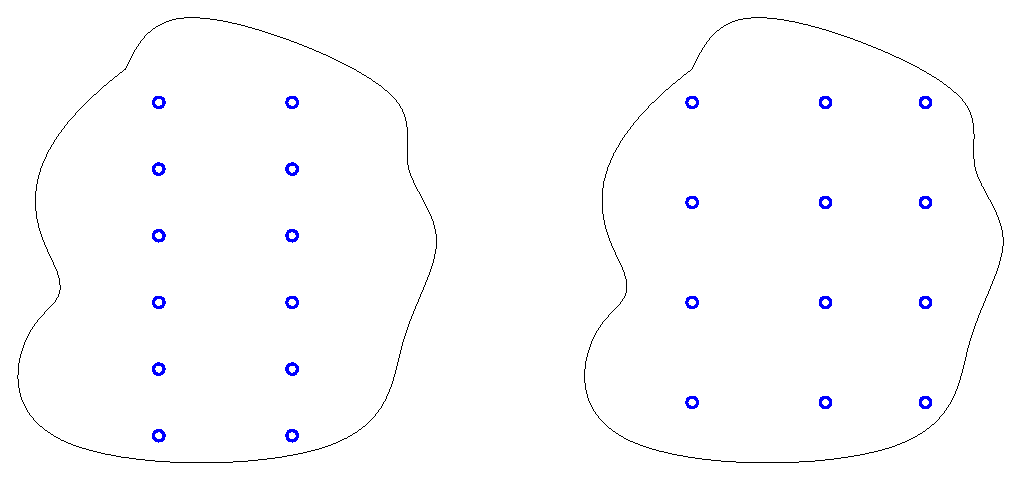
\includegraphics[scale=0.5]{motivation/deployment-configuration.eps}
\end{figure}
We have 12 sensors which we can \emph{deploy} in various configurations.
\end{frame}
%%
\begin{frame}[label=motivation7]{Deployment and full coverage}
Is it that simple?

\begin{figure}[b]
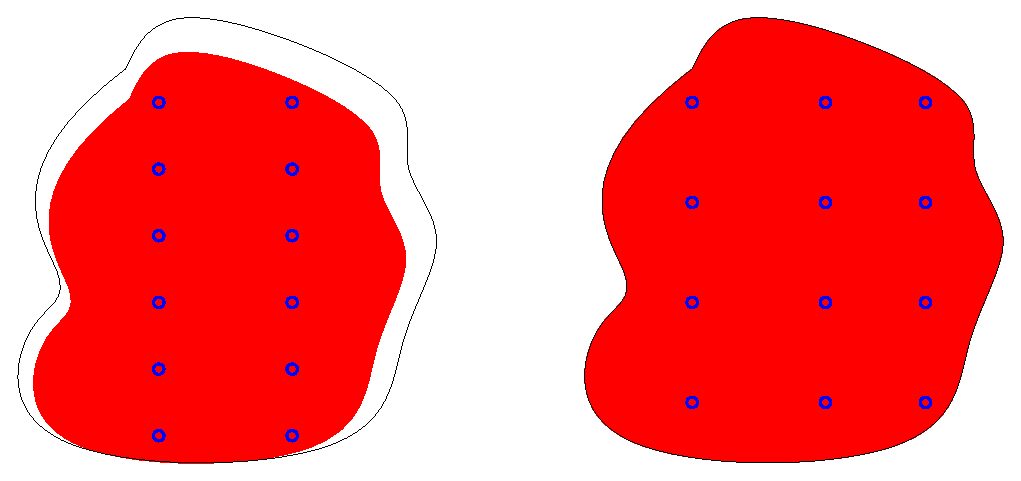
\includegraphics[scale=0.5]{motivation/deployment-configuration-partial-full-example.eps}
\end{figure}
One configuration results with full coverage, while the other one doesn't.
\end{frame}
%%
\begin{frame}[label=motivation8]{Partial Coverage}
There exists a deployment with 12 sensors which can cover the area. What if we only have 6 sensors?

\begin{figure}[b]
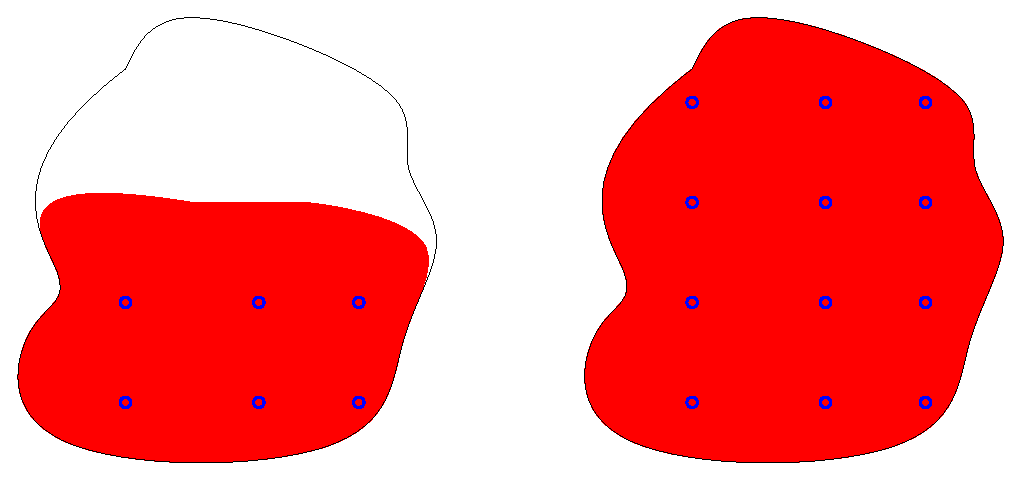
\includegraphics[scale=0.5]{motivation/deployment-configuration-partial-no-enough-sensors.eps}
\end{figure}
There isn't a configuration that can provide full coverage!
\end{frame}
%%
\begin{frame}[label=motivation9]{Making it a bit more interesting...}
Let's say that we want to maintain coverage on a specific area, due to:
\begin{itemize}
\item Connection to home base
\item Maintain surveillance on a target
\begin{figure}[b]
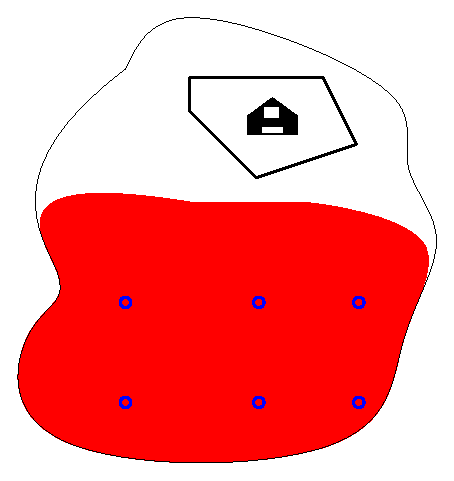
\includegraphics[scale=0.4]{motivation/deployment-configuration-coverage-constraint.eps}
\end{figure}
We have to take this into account when we build our coverage \emph{strategy}.
\end{itemize}
\end{frame}
%%
\begin{frame}[label=motivation10]{Partial Coverage Strategy}
Dealing with partial coverage - many possible behaviours:
\begin{itemize}
\item Set of trajectories $^{1,2}$
\item \emph{Tiling the area}$^{3}$

\end{itemize}

By choosing any strategy, a \emph{coverage controller}$^3$ must be provided.

\footnotetext[1]{\tiny Atinç, G. M., Stipanović, D. M., Voulgaris, P. G., \& Karkoub, M. (2013). Supervised coverage control with guaranteed collision avoidance and proximity maintenance. Proceedings of the IEEE Conference on Decision and Control, 3463–3468.}
\footnotetext[2]{\tiny Hussein, I. I., \& Stipanovic, D. M. (2007). Effective Coverage Control for Mobile Sensor Networks With Guaranteed Collision Avoidance. IEEE Transactions on Control Systems Technology, 15(4), 642–657.}
\footnotetext[3]{\tiny Cortes, J., \& Martinez, S. (2004). Coverage control for mobile sensing networks.  IEEE Transactions on Robotics and Automation, 20(2), 243-255.}
\footnotetext[4]{\tiny Cassandras, C. G., \& Li, W. (2005). Sensor Networks and Cooperative Control. Decision and Control, 2005 and 2005 European Control Conference. CDC-ECC ’05. 44th IEEE Conference On, 4237–4238.}
\end{frame}
%%
\begin{frame}[label=motivation12]{Partitioning as a strategy}
\emph{Partitioning} (or tiling) an area - cover a small part of the area for a set of time intervals.
\begin{itemize}
\item Main benefit - provide coverage of a subset of an area constantly.
\end{itemize}

$[$Cortes2004$]$ provided a controller that knows how to partition an area and provide coverage, using Centroidal Voronoi Tessellations$^1$.

\begin{figure}[b]
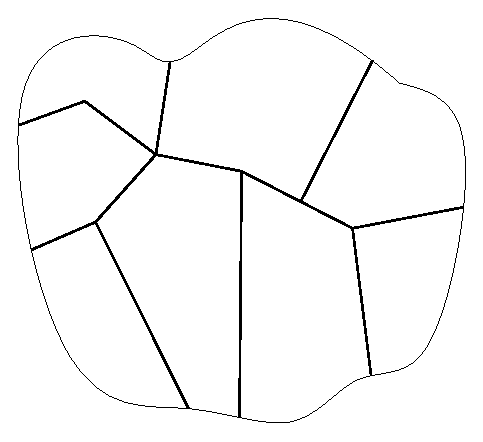
\includegraphics[scale=0.4]{motivation/partitioning.eps}
\end{figure}

\footnotetext[1]{\tiny Du, Q., Faber, V., \& Gunzburger, M., “Centroidal Voronoi Tessellations: Applications
and Algorithms,” SIAM Review, Vol. 41, No. 4, 1999, pp. 637–676.}
\end{frame}

%%% Problem Formulation %%%
\subsection[Problem Formulation]{}
\begin{frame}[label=probformulation1]{Problem Formulation}
\begin{itemize}
\item There is some area $A \in \rR^{2}$ That we aim to cover.
\item A sub-area $A_{m} \subset A$ must be partially covered always (e.g. ground station).
\item There exist a set of \textbf{mobile} sensors $S = \left\{s_1 \ldots s_n\right\}$ located in positions $p_i(t) \in \mathbb{R}^2$ (for $i=1,\ldots,n$) at time $t$.
\begin{itemize}
\item The mobile sensors are modelled using integrator dynamics $\dot{p_i}(t) = u$.
\item Each sensor can cover an area described by the abstract set $C_i(p_i(t)) \subset \mathbb{R}^2$.
\end{itemize}
\end{itemize}
\end{frame}
%%
\begin{frame}[label=probformulation2]{Problem Formulation}
\begin{itemize}
\item A configuration $c$ at time $t$ is the stack of the sensor positions at time $t$,
\begin{equation*}
c\left(t\right) = \bmat{
p_{1}^{T}\left(t\right)&\cdots&p_{n}^{T}\left(t\right)}^{T}\in\mathbb{R}^{2n}
\end{equation*}
\begin{itemize}
\item The coverage of a configuration $D\left( c\left( t \right) \right) = \cap C_i(p_i(t))$.
\end{itemize}
\end{itemize}
\begin{block}{Assumption}
$D\left( c\left( t \right) \right) \subset A$ - a single configuration \emph{can't} provide full coverage!
\end{block}
\end{frame}
%%
\begin{frame}[label=probformulation2]{Problem Formulation}
\begin{itemize}
%\item A partition $j$ of the area $A$ is $pr_{j} \subset A$
\item The partitioning of $A, PR\left( A \right)$, is a finite set built from $n$ partitions $pr_{1},\ldots,pr_n$:
\begin{itemize}
\item The partitions does not intersect one with each other,
\item The union of the $n$ partitions is exactly the area $A$.
\end{itemize}
\begin{equation*}
PR\left( A \right) = \{ pr_{j} \mid \forall i \neq j,\textbf{ } pr_{i}\cap pr_{j} = \emptyset \textbf{ and }\cup pr_{j} = A \}
\end{equation*}
\end{itemize}
\end{frame}
%%
\begin{frame}[label=probformulation2]{Problem Formulation}
\begin{problem} \label{GeneralProblem}
\begin{enumerate}
\item Find partitioning such that for each partition $j, pr_{j} \cap A_m \neq \emptyset$ 
\item Find a deployment controller, such that for a given partition $pr_j, lim_{(t\rightarrow \infty)}D(c(t)) \subseteq PR(A)$
\end{enumerate}
\end{problem}
\pause
In more simple words:
\begin{itemize}
\item Find partitioning such that every partition intersect with $A_m$,
\item In some time, there is a full coverage of a partition $pr_j$, for $j=1,\ldots, n$.
\end{itemize}
\end{frame}

%%%%%%%%%%%%%%%%%%%%%%%%%%%%%%%%%%%%%%%%%%
%%%%%%%%%%%%% MATH BACKGROUND %%%%%%%%%%%%
%%%%%%%%%%%%%%%%%%%%%%%%%%%%%%%%%%%%%%%%%%

\section[Mathematical Background]{Mathematical Background}
%%% Voronoi Partitioning %%%

\subsection[Voronoi Partitioning]{}
\begin{frame}[label=vorpart1]{Voronoi Partitioning}
\begin{center}
A short story about a postal company that wants to become more efficient...
\end{center}
\begin{figure}
\centering

\includegraphics[scale=0.1]{background/israelpost-logo.png}
\end{figure}
\end{frame}
%%
\begin{frame}[label=vorpart2]{Voronoi Partitioning}
The Voronoi Diagram of a region $\Omega \subset \rsqr$ is the set of partitions $\mathcal{V} = \left\{V_{i} \mid \cup V_{i} = \Omega\right\}$, generated by the generators $\mathcal{Z} = \{z_1,\ldots,z_n\mid z_{i} \in \Omega\}$, such that
\begin{equation*} \label{Voronoi Definition}
V_{i} = \{q\in\Omega \mid \lVert q - z_i \rVert \leq \lVert q - z_j \rVert \forall z_i,z_j\in\mathcal{Z}\},
\end{equation*}
where $V_{i}$ corresponds to the $i$-th element of $\mathcal{Z}$, and $\lVert \cdot \rVert$ denotes the Euclidean distance.
\end{frame}
%%
\begin{frame}[label=vorpart3]{Voronoi Partitioning}
A rough example:
\begin{center}
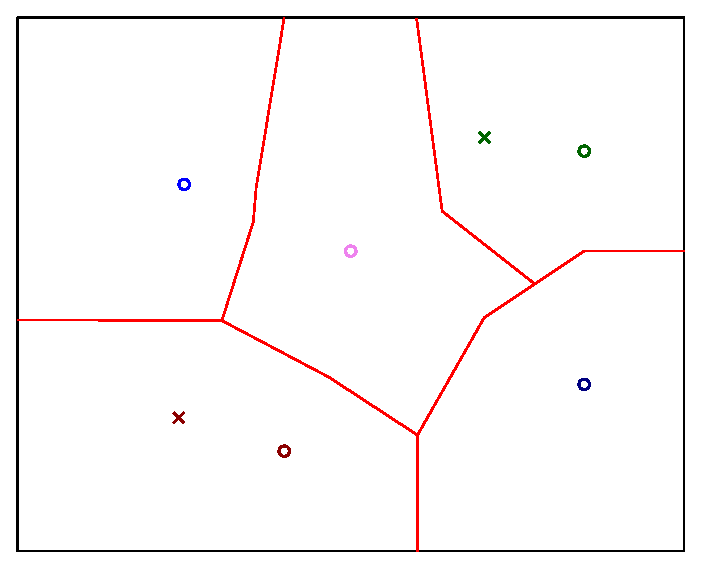
\includegraphics[scale=0.6]{background/Voronoi-example.eps}
\end{center}
Circles - generators, crosses - some point inside the appropriate partition.
\end{frame}
%%
\begin{frame}[label=centvorpart1]{Central Voronoi Tessellations}
\begin{center}
Building a new neighbourhood!
\begin{figure}
\centering
\includegraphics[scale=0.05]{background/sketch.jpg}
\end{figure}
\end{center}
\end{frame}
%%
\begin{frame}[label=centvorpart2]{Central Voronoi Tessellations}
Let us define a density function, $\rho_i$, for each Voronoi partition $V_{i}$. Then, we can define the center of mass for each partition as
\begin{equation*}
z_{i}^{*} = \frac{\int_{V_{i}}y\rho(y)dy}{\int_{V_{i}}\rho(y)dy}.
\end{equation*}
If a generator $z_{i} = z_{i}^{*} \, \forall \,V_{i}$, we call this partitioning a \emph{centroidal Voronoi tessellation} (CVT).
%%
Common examples for density function:
\begin{itemize}
\item $\rho(y) = \mathcal{N}\left( \mu, \sigma ^2 \right)$ (Gaussian distribution)
\item $\rho(y) = 1$
\end{itemize}
\end{frame}
%%
\begin{frame}[label=centvorpart3]{Central Voronoi Tessellations}
How it looks like?
\begin{center}
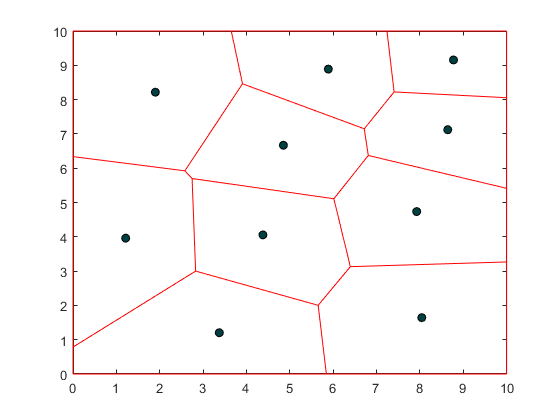
\includegraphics[scale=0.5]{background/central-Voronoi-example.png}
\end{center}
\end{frame}
%%
\begin{frame}[label=lloydsalg1]{Lloyd's Algorithm}
How do we calculate CVT?
\begin{algorithm}[H]
\caption{Lloyd's Algorithm} \label{LloydAlgo}
\begin{algorithmic}[1]
\State Calculate the Voronoi diagram for the current agents positions.
\State Calculate the center of mass for every cell.
\State Move the agents to the center of mass.
\State Repeat until convergence.
\end{algorithmic}
\end{algorithm}
\end{frame}
%%
\begin{frame}[label=lloydsalg2]{Lloyd's Algorithm}
So how do we calculate it?\\
Step 1:
\begin{figure}
\centering
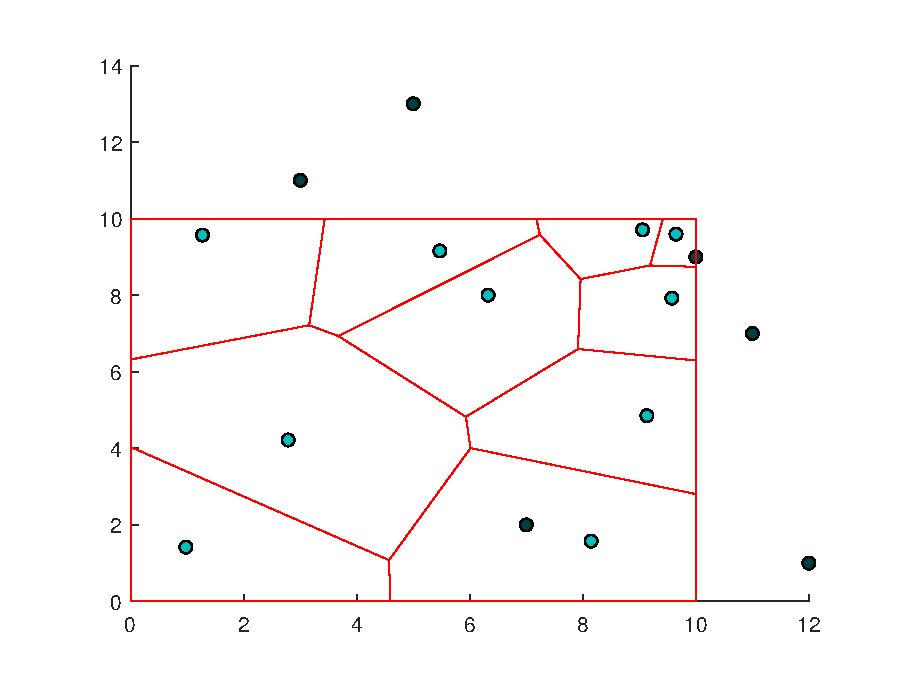
\includegraphics[scale=0.4]{background/cvt-calc-step1.eps}
\end{figure}
Black - initial guess, turquoise - after first iteration
\end{frame}
%%
\begin{frame}[label=lloydsalg3]{Lloyd's Algorithm}
Step 2:
\begin{figure}
\centering
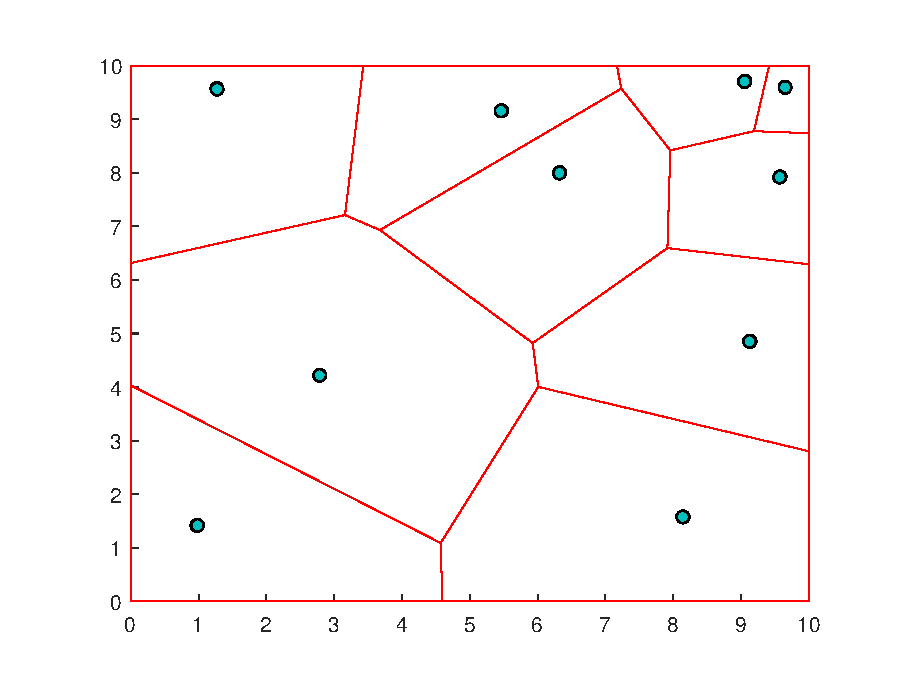
\includegraphics[scale=0.4]{background/cvt-calc-step2.eps}
\end{figure}
Black - first iteration solution, turquoise - after second iteration
\end{frame}
%%
\begin{frame}[label=lloydsalg4]{Lloyd's Algorithm}
Step 2 - zoom in:
\begin{figure}
\centering
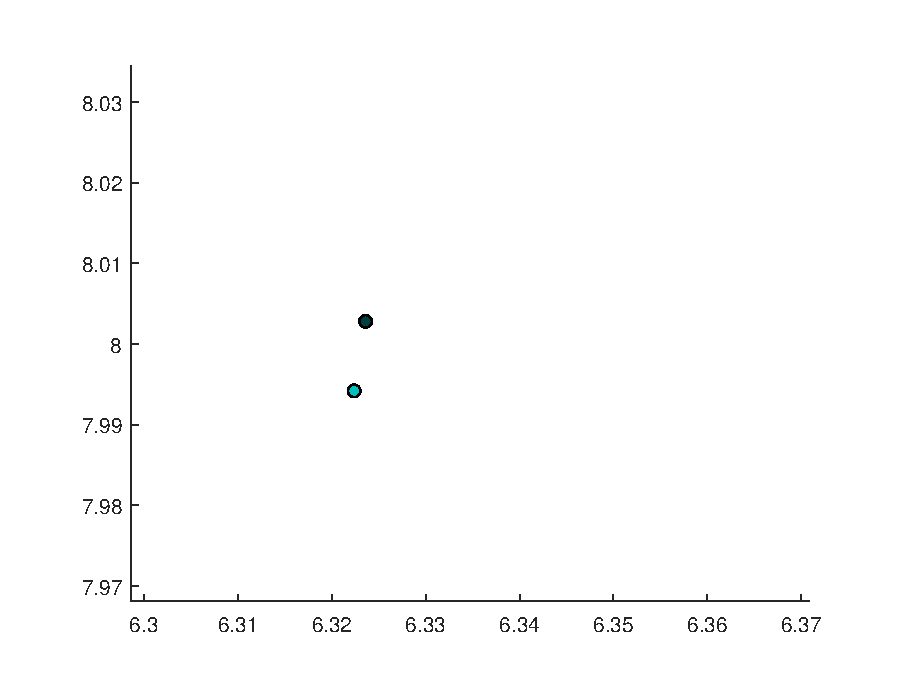
\includegraphics[scale=0.4]{background/cvt-calc-step2-zoom.eps}
\end{figure}
Almost converged...
\end{frame}
%%
\begin{frame}[label=lloydsalg5]{Lloyd's Algorithm}
Asymptotically convergence to CVT:
\begin{figure}
\centering
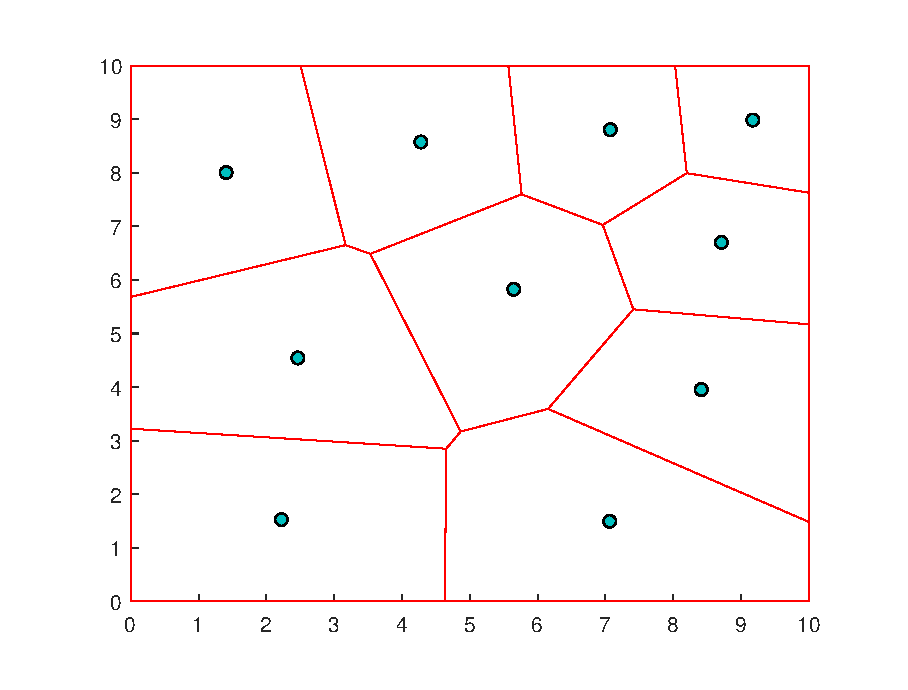
\includegraphics[scale=0.4]{background/cvt-calc-stepn.eps}
\end{figure}
\end{frame}
%%
\begin{frame}[label=lloydsalg6]{Lloyd's Algorithm}
[Cortes2004] proposed a continuous time controller for Lloyd's algorithm. If we define agent $i$ position as $p_i$ and the $i$'s partition centroid as $C_{V_{i}}$, then for some proportional constant $k_{p}$, the controller can be defined as:
\begin{equation*} \label{Lloyds contoller}
u_{i} = -k_{p}\left( p_i - C_{V_{i}} \right)
\end{equation*}

\begin{figure}[b]
\centering
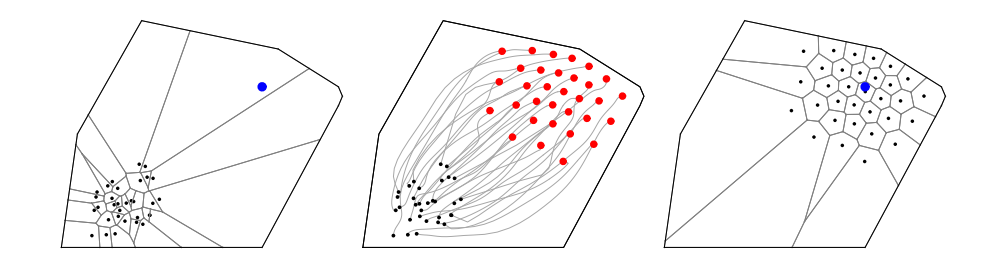
\includegraphics[scale=0.3]{background/Lloyds-alg-from-cortes.png}
\caption{A simulation from [Cortes2004] with 32 agents and Gaussian density function}
\end{figure}
\end{frame}
%%
\begin{frame}[label=lloydsalg7]{Lloyd's Algorithm}
Another important result in [Cortes2004] is that this controller is locally asymptotically stable. Proof is given in the paper using the direct Lypunov methos, using the following potential function:
\begin{equation*}
\mathcal{H_{V}}\left( P \right) = \sum_{i=1}^{n} J_{V_i,C_{V_i}} + \sum_{i=1}^{n} M_{V_i} \norm{p_i - C_{V_i}}^2
\end{equation*}
Where:
\begin{itemize}
\item P - the set of the agents positions
\item $V_i$ - the $i$'th Voronoi partition
\item $J_{V_i,C_{V_i}}$ - the polar moment of inertia of $V_i$ about its centroid $C_{V_i}$
\item $M_{V_i}$ - the $i$'th partition "mass"
\end{itemize}
\end{frame}

%%%%%%%%%%%%%%%%%%%%%%%%%%%%%%%%%%%%%%%%%%
%%%%%%%%%%%%% PROBLEM SOLUTION %%%%%%%%%%%
%%%%%%%%%%%%%%%%%%%%%%%%%%%%%%%%%%%%%%%%%%

\section[Problem Solution]{Problem Solution}
%%% PLA %%%
\subsection[Projected Lloyd's Algorithm]{}
\begin{frame}[label=probreminder]{Problem reminder}
So what were we trying to do (in simple words)?
\begin{block}{Reminder}
\begin{enumerate}
\item Partition the area $A$, such that any partition will intersect with some sub-area $A_m$.
\item For each partition, find some deployment strategy.
\end{enumerate}
\end{block}\pause
$[$Cortes2004$]$ came up with a solution for the second issue. But what about the first one?
\end{frame}
%%
\begin{frame}[label=solproposal]{Projection}
A possible solution - After calculating the center of mass of each cell, \emph{project} the results onto the set $A_m$.
\\ \pause
\begin{block}{Projection - Definition}
A linear transformation $P$ from a vector space to itself such as $P^2 = P$. In other words, the transformation $P$ is idempotent.
\end{block}
We will project using Euclidean distance, and mark the projection of the scalar $a$ as $\textsc{proj}(a)$.
\end{frame}
%%
\begin{frame}[label=solprojectionexample]{Projection example}
\begin{figure}
\centering
\includegraphics<1>[scale=0.7]{Problem-solution/projection-before.eps}
\includegraphics<2>[scale=0.7]{Problem-solution/projection-after.eps}
\end{figure}
\end{frame}
%%
\begin{frame}[label=projlloydsalgo]{Projected Lloyd's Algorithm}
\begin{algorithm}[H]
\caption{Projected Lloyd's Algorithm (PLA)}\label{ProjLloydsAlgorithm}
\begin{algorithmic}[1]
\State Calculate the Voronoi diagram for the current agents positions.
\State Calculate the center of mass for every cell.
\State Project the center of mass of every cell to the area constraint limiting polygon.
\State Move the agents the projected center of mass.
\State Repeat until converge.
\end{algorithmic}
\end{algorithm}
\end{frame}
%%
\begin{frame}[label=projlloydsalgoexample]{Projected Lloyd's Algorithm Example}
Assume that we have an area $A$ and some sub-area $A_m$:
\begin{figure}
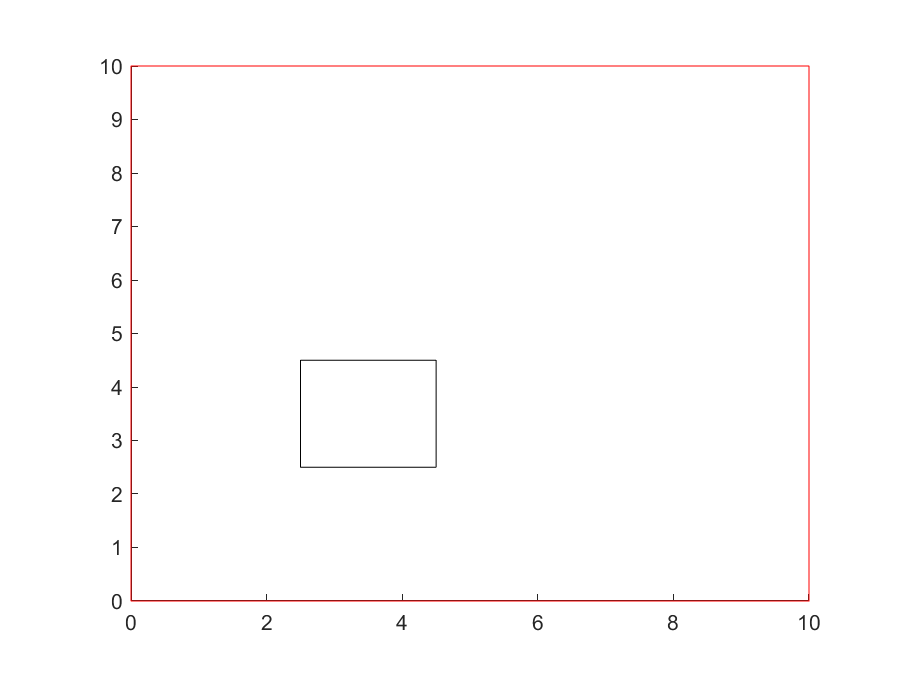
\includegraphics[scale=0.6]{Problem-solution/PLA-example-empty.eps}
\end{figure}
\end{frame}
%%
\begin{frame}[label=projlloydsalgo3]{Projected Lloyd's Algorithm}
\begin{columns}
\column{0.5\textwidth}
\begin{figure}[!H]
  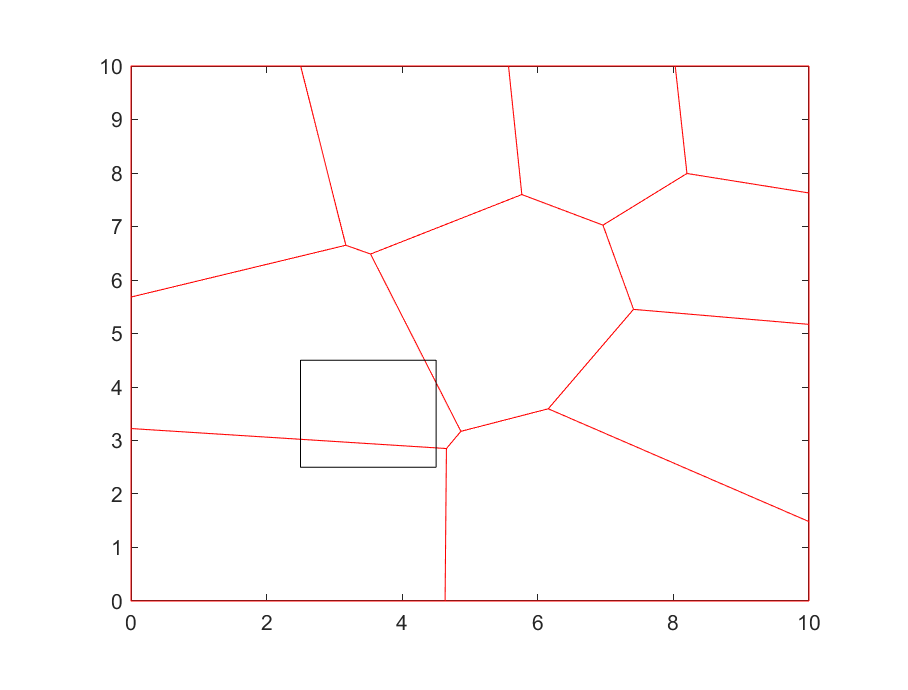
\includegraphics[scale=0.43]{Problem-solution/proj-lloyds-off.eps}
  \caption*{CVT using Lloyd's Algorithm}
\end{figure}
\column{0.5\textwidth}
\begin{figure}[!H]
  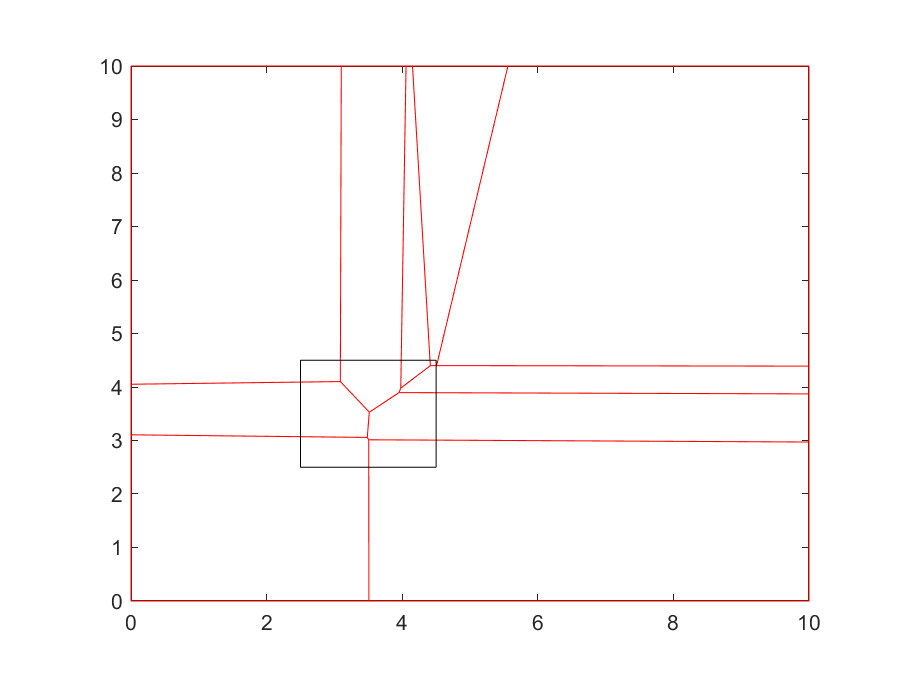
\includegraphics[scale=0.43]{Problem-solution/proj-lloyds-on.eps}
  \caption*{Partitioning using PLA}
\end{figure}
\end{columns}

\end{frame}
%%
\begin{frame}[label=projlloydsalgotheorem]{Projected Lloyd's Algorithm}
PLA in continuous time controller form:
\begin{equation*} \label{ProjectedLloydsContol}
u_{i} = -k_{p}\left( p_i - \textsc{proj}\left( C_{V_{i}} \right) \right)
\end{equation*} 

\begin{theorem}
The projected Lloyd's Algorithm is locally asymptotically stable
\end{theorem}

Proof of stability is using the direct Lyapunov method, with a potential function being very similar to the one proposed in [Cortes2004]:
\begin{equation*}
\mathcal{H_{V}}\left( P \right) = \sum_{i=1}^{n} J_{V_i,C_{V_i}} + \sum_{i=1}^{n} M_{V_i} \norm{p_i - \textsc{proj}\left( C_{V_i}\right)}^2
\end{equation*}
\end{frame}

%%% Problem solution algorithm %%%
\subsection[Problem Solution Algorithm]{}
\begin{frame}[label=probsolalg1]{Problem Solution Algorithm}
So far:
\begin{itemize}
\item Covering a given area using Voronoi partitioning - \textbf{Solved} ([Cortes2004]).
\item Partition and area such that the coverage constraint is fulfilled - \textbf{Solved} (PLA).
\end{itemize}

Therefore, we are ready for the problem solution algorithm...
\end{frame}

\begin{frame}[label=probsolalg2]{Problem Solution Algorithm}
\begin{algorithm}[H]
\caption{Problem Solution Algorithm}\label{GeneralProbSolution}
\begin{algorithmic}[1]
\State Using some random initial guess, partition the whole area using PLA.
\State For each partition (assuming that the agents can actually cover each partition with their coverage radius), calculate the CVT. The initial positions for the CVT calculation is the previous partition CVT.
\end{algorithmic}
\end{algorithm}
\end{frame}

%%
\begin{frame}[label=planotice]{Some Characteristics}
\begin{itemize}
\item This form of PLA (and also Lloyd's algorithm) is centralized!
\item The calculation of the Voronoi partitions converges into a local minima and not a global one.
\item Lloyd's algorithm A converges into a local minima. PLA \emph{isn't} an optimal solution!
\end{itemize}

\end{frame}
%%% Problem simulations %%%
\subsection[Simulations]{}
\begin{frame}[label=plasim1]{Simulation \#1}
3 agents, 3 partitions, PLA deactivated.
\begin{figure}
\centering
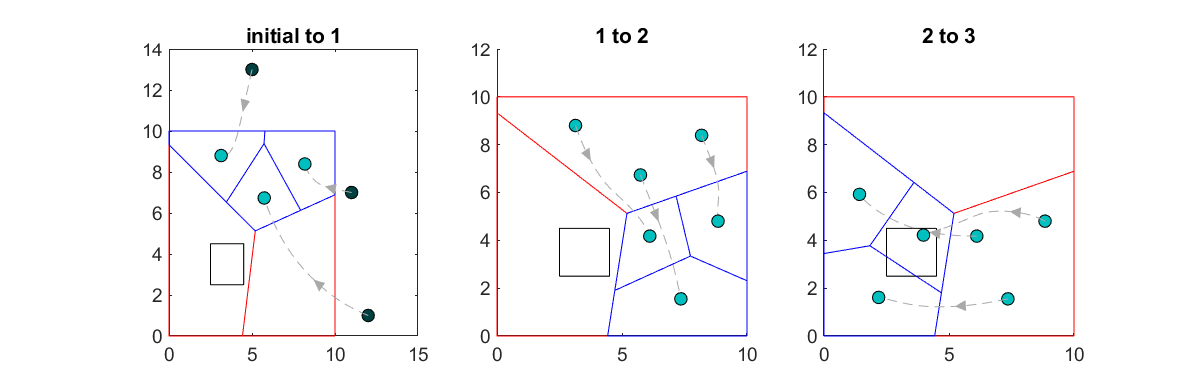
\includegraphics[scale=0.6]{sim/sim1-3agents-3partitions-noPLA.eps}
\end{figure}
\end{frame}
%%
\begin{frame}[label=plasim2]{Simulation \#2}
3 agents, 3 partitions, PLA activated.
\begin{figure}
\centering
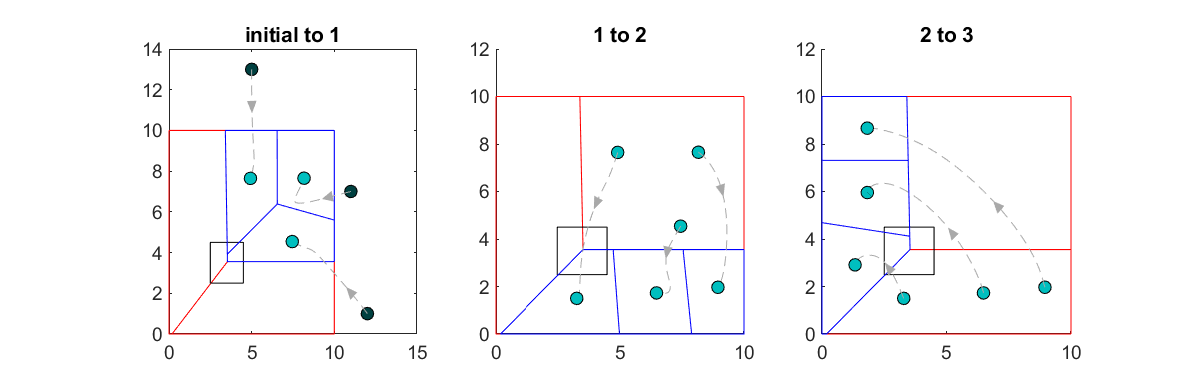
\includegraphics[scale=0.6]{sim/sim2-3agents-3partitions-PLA.eps}
\end{figure}
\end{frame}

%%%%%%%%%%%%%%%%%%%%%%%%%%%%%%%%%%%%%%%%%%
%%%%%%%%%%%% Formation Control %%%%%%%%%%%
%%%%%%%%%%%%%%%%%%%%%%%%%%%%%%%%%%%%%%%%%%

%%% Motivation%%%
\section[Formation Control and PLA]{}
\begin{frame}[label=onemorething]{One more thing...}
\begin{itemize}
\item<1-> Problem solved.
\item<2-> What if maintaining spatial properties is also needed? \begin{itemize}
	\item<2-> Geolocation
	\item<2-> communications
\end{itemize}
\item<3-> Incorporate formation control into existing algorithms!
\end{itemize}
\end{frame}

%%% Math background %%%
\subsection[Distance-Based Formation Control]{}
\begin{frame}[label=distanceformation1]{Formation Control}
The concept of distance-based formation control is well researched$^{1,2}$.

\begin{columns}
\column{0.5\textwidth}
\begin{itemize}
\item<2-> We have agents $1 \ldots n$ on positions $p_{i}$.
\item<3-> Only $\varepsilon$ agents can share information ("connected by edge").
\item<4-> Goal - agents $i,j (i \neq j)$ will be at distance $d_{ij}$.
\end{itemize}

\column{0.5\textwidth}
\begin{center}
\includegraphics<2>[scale=0.6]{formation-control/formation-positions.eps}
\includegraphics<3>[scale=0.6]{formation-control/rigid-formation-connections.eps}
\includegraphics<4>[scale=0.6]{formation-control/rigid-formation-connections-dist.eps}
\end{center}
\end{columns}
\footnotetext[1]{\tiny L. Krick, M.E. Broucke \& B.A. Francis (2009) Stabilisation of infinitesimally rigid formations of multi-robot networks, International Journal of Control, 82:3, 423-439.}
\footnotetext[2]{\tiny K. Oh \& H. Ahn, "Distance-based formation control using euclidean distance dynamics matrix: Three-agent case," Proceedings of the 2011 American Control Conference, San Francisco, CA, 2011, pp. 4810-4815.}
\end{frame}
%%
\begin{frame}[label=distanceformation2]{Formation Control}
A formation has a potential, defined by:
\begin{equation*}
F(p) = \frac{1}{4}\sum_{k=1}^{\varepsilon}\left( \norm{e_k}^2 - d_{k}^{2} \right)
\end{equation*}
Where $e_k$ is the actual distance of edge $k$, and $d_k$ is the required distance of this edge.

The proposed controller is a gradient dynamics controller:
\begin{equation*}
\dot{p} = -\nabla F(p)
\end{equation*}

\end{frame}
%%
\begin{frame}[label=distanceformation3]{Formation Control}
For a single agent $p_i$, the controller will have the following form:
\begin{equation*}
    \dot{p_{i}} = -\sum_{i \sim j} \left( \norm{p_{i} - p_{j}}^{2} - d_{ij}^2 \right) \left( p_{i} - p_{j} \right)
    \label{formation controller}
\end{equation*}

To prove stability - we will once again use the direct Lyapunov method. This time, with the potential function as the candidate Lyapunov function.

\end{frame}

%%% Lloyd's and formation %%%
\subsection[Lloyd's Algorithm and Formation Control]{}
\begin{frame}[label=lloydsandformation1]{Lloyd's Algorithm and Formation Control}
Both Lloyd's algorithm controller and distance based formation controller:
\begin{itemize}
\item Locally asymptotically stable.
\item Gradient descent controllers.
\end{itemize} 
We propose to simply combine them with some coefficient $0 \leq \alpha \leq 1$:
\begin{align}
    u_{i} = \alpha \left(-k_{p}\left( p_i -C_{V_{i}} \right)\right) +
    \left( 1-\alpha \right)\left[-\sum_{i \sim j} \left( \norm{p_{i} - p_{j}}^{2} - d_{ij}^2 \right) \left( p_{i} - p_{j} \right)  \right] 
    \label{Combined Controller}
\end{align}
\end{frame}
%%
\begin{frame}[label=lloydsandformation2]{Lloyd's Algorithm and Formation Control}
\begin{theorem}
The combined controller is Locally Asymptotically Stable
\end{theorem}

To prove this, using a direct Lyapunov function, use the following candidate Lyapunov function:
\begin{align*}
        V_{c}\left(P\right) &= \alpha\left[ \sum_{i=1}^{n} J_{V_i,C_{V_i}} + \sum_{i=1}^{n} M_{V_i} \norm{p_i - C_{V_i}}^2 \right] +\\
        &(1-\alpha) \left[ \frac{1}{4}\sum_{k=1}^{\varepsilon}\left( \norm{e_k}^2 - d_{k}^{2} \right) \right]
\end{align*}

* In the same way, we can show it works with the PLA.
\end{frame}
%%
\begin{frame}[label=lloydsandformation3]{"Disclaimer"}
\begin{alertblock}{Notice!}
We do not supply a condition to both maintain the required spatial formation \textbf{and} the original problem requirements.
\end{alertblock}

Moreover, Since this problem is highly non-linear, it is hard to characterize what are the equilibrium points.
\pause
\begin{Proposition}
Let us assume that there exists a (CVT) with $C_{V_{i}}$ such that $\forall i \neq j, \norm{C_{V_{i}} - C_{V_{j}}}^{2} = d_{ij}^{2}$. Then, there exists an equilibrium such that $p_{i} = C_{V_{i}}$, which is locally asymptotically stable with the "combined controller" dynamics.
\end{Proposition}
\end{frame}
%%% Problem simulations %%%
\subsection[Simulations]{}
\subsection[Simulations]{}
\begin{frame}[label=formsim1]{Simulation \#1}
Defined a triangular shaped formation:
\begin{figure}
\centering
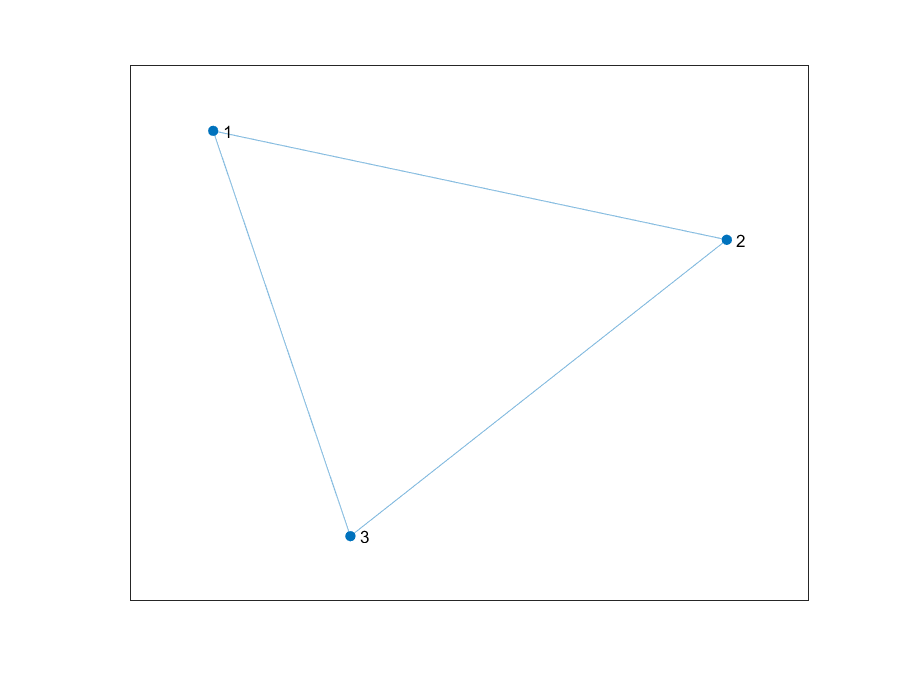
\includegraphics[scale=0.6]{sim/sim-formationshape.eps}
\end{figure}
\end{frame}
%%
\begin{frame}[label=plasim2]{Simulation \#2}
3 agents, 3 partitions, PLA deactivated, with Triangular formation.
\begin{figure}
\centering
\includegraphics<1>[scale=0.6]{sim/sim1-3agents-3partitions-noPLA.eps}
\includegraphics<2>[scale=0.6]{sim/sim3-3agents-3partitions-noPLA-formation.eps}
\end{figure}
\end{frame}
%%
\begin{frame}[label=plasim3]{Simulation \#2}
3 agents, 3 partitions, PLA activated, with Triangular formation.
\begin{figure}
\centering
\includegraphics<1>[scale=0.6]{sim/sim2-3agents-3partitions-PLA.eps}
\includegraphics<2>[scale=0.6]{sim/sim4-3agents-3partitions-PLA-formation.eps}
\end{figure}
\end{frame}

%%%%%%%%%%%%%%%%%%%%%%%%%%%%%%%%%%%%%%%%%%
%%%%%%%%%%%%%% CONCLUSIONS %%%%%%%%%%%%%%%
%%%%%%%%%%%%%%%%%%%%%%%%%%%%%%%%%%%%%%%%%%

\section[Conclusions]{Conclusions}
\subsection[Conclusions]{}
\begin{frame}[label=conclusions]{Conclusions}
\begin{itemize}
\item A modified algorithm for partitioning an area with sub-area constraint was introduced (PLA).
\begin{itemize}
\item A centralized method.
\item The method is locally asymptotically stable.
\end{itemize}
\item It is possible to combine Lloyd's algorithm with distance-based formation control to achieve spatial properties.
\end{itemize}
\end{frame}
%%
\subsection[Future Work]{}
\begin{frame}[label=futurework]{Future Work}
\begin{itemize}
\item Distributed version.
\item Developing the combination of formation controller and Lloyd's algorithm.
\end{itemize}
\end{frame}
%%
\subsection[Acknowledgements]{}
\begin{frame}[label=acknowledgements]{Acknowledgements}
\begin{itemize}
\item Associate Professor Daniel Zelazo
\end{itemize} \pause
This work will be presented at the 59'th Israel Annual Conference on Aerospace Sciences
\end{frame}
%%
\subsection[Thank you]{}
\begin{frame}{}
  \centering \Large
  \emph{Thank you}
\end{frame}
\end{document}